% ============================================================
%  第一章 控制系统基础知识
%  整理自《控制工程基础》读书笔记
% ============================================================
\section{增益（Gain）}
\begin{definition}[增益]
	增益是一个比例值，显示了稳态时输入信号大小与输出信号大小之间的关系。许多系统提供改变增益的方法，从而为系统提供或多或少的“功率（power）”。
\end{definition}

下图所示系统，由于输出是输入幅度的两倍，因此系统的增益为 $K=2$。

\begin{figure}[htbp]
	\centering
	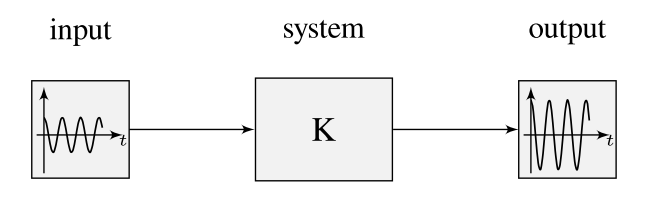
\includegraphics[width=0.55\textwidth]{Figure/增益为K=2的系统的演示.png}
	\caption{增益为 $K=2$ 的系统演示}
	\label{fig:gain-K2}
\end{figure}

\section{方框图（Block diagrams）}
方框图是设计与分析控制系统的有力工具，可被系统地操纵和简化。其一般形式如下图所示。

\begin{figure}[htbp]
	\centering
	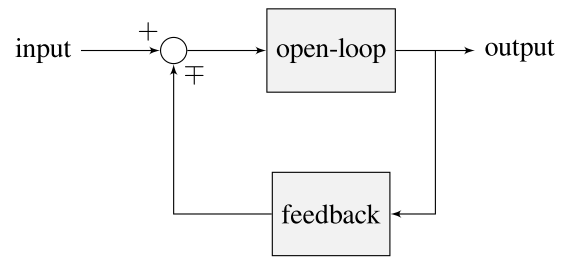
\includegraphics[width=0.7\textwidth]{Figure/带命名法的框图.png}
	\caption{带命名法的方框图}
	\label{fig:block-named}
\end{figure}

\begin{definition}[开环增益]
	开环增益是从输入（圆）处的和节点到输出支路的总增益。若把反馈回路断开，这就是系统的增益。
\end{definition}

\begin{definition}[反馈增益]
	反馈增益是从输出返回到输入和节点的总增益。求和节点的输出是其输入的总和。
\end{definition}

\subsection{级联块（Cascaded blocks）}
表示关系：
\begin{equation}
	Y = (P_1P_2)\,X .
	\label{eq:cascade}
\end{equation}
图示形式如下。

\begin{figure}[htbp]
	\centering
	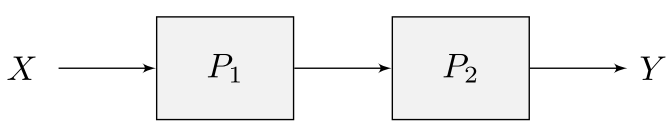
\includegraphics[width=0.55\textwidth]{Figure/级联块.png}\hfill
	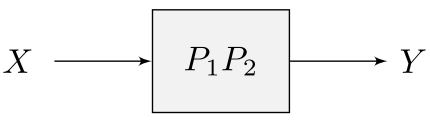
\includegraphics[width=0.4\textwidth]{Figure/简单级联块.png}
	\caption{级联块的两种表示}
	\label{fig:cascade}
\end{figure}

\subsection{并行组合块（Combining blocks in parallel）}
表示关系：
\begin{equation}
	Y = P_1X \pm P_2X .
	\label{eq:parallel}
\end{equation}
图示形式如下。

\begin{figure}[htbp]
	\centering
	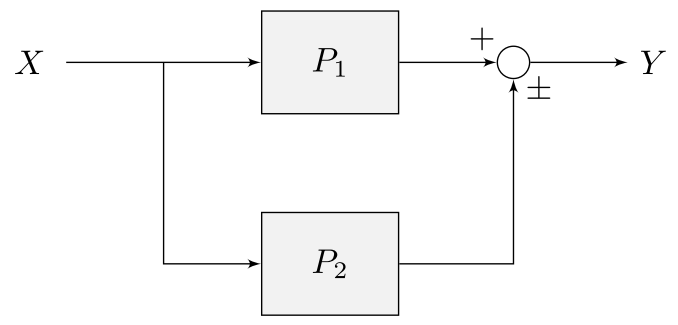
\includegraphics[width=0.55\textwidth]{Figure/并行块.png}\hfill
	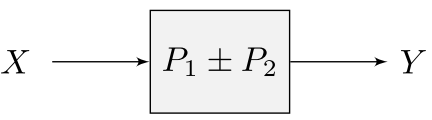
\includegraphics[width=0.4\textwidth]{Figure/简单并行块.png}
	\caption{并行组合块的两种表示}
	\label{fig:parallel}
\end{figure}

\subsection{从前馈循环中删除块}
表示关系：
\begin{equation}
	Y = P_1X \pm P_2X .
	\label{eq:feedforward}
\end{equation}
图示关系如下。

\begin{figure}[htbp]
	\centering
	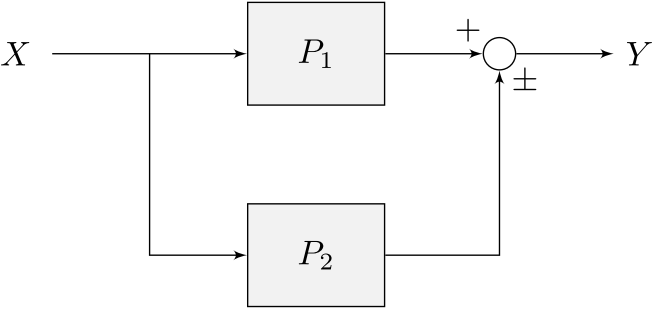
\includegraphics[width=0.5\textwidth]{Figure/前馈环.png}\hfill
	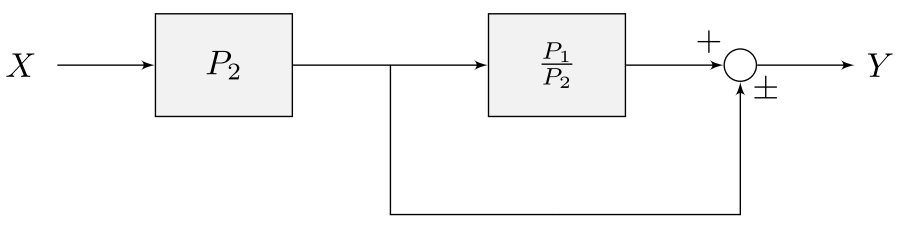
\includegraphics[width=0.5\textwidth]{Figure/变换的前馈环.png}
	\caption{前馈环及其变换}
	\label{fig:feedforward}
\end{figure}

\subsection{消除反馈回路}
表示关系：
\begin{equation}
	Y = P_1\bigl(X \mp P_2Y\bigr) .
	\label{eq:feedback}
\end{equation}
图示关系如下。

\begin{figure}[htbp]
	\centering
	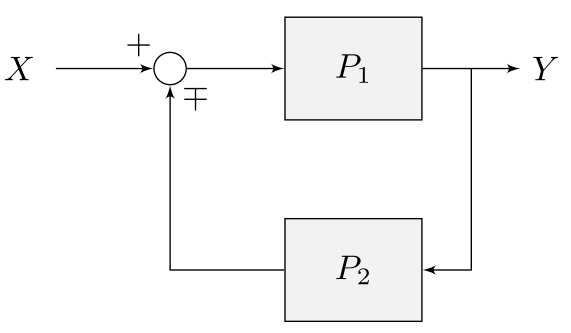
\includegraphics[width=0.5\textwidth]{Figure/反馈环.png}
	\caption{反馈环}
	\label{fig:feedback-orig}
\end{figure}

\begin{figure}[htbp]
	\centering
	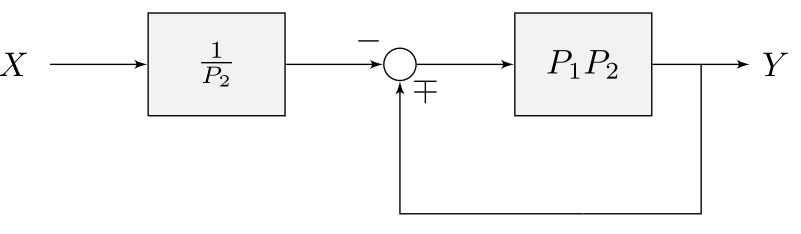
\includegraphics[width=0.85\textwidth]{Figure/变换的反馈环.png}
	\caption{反馈环的变换}
	\label{fig:feedback-trans}
\end{figure}

\section{开环和闭环系统}
\begin{definition}[Plant]
	放置被控制的执行器的系统或集合称为 \emph{Plant}。
\end{definition}

\begin{definition}[控制器]
	\emph{控制器}（\emph{Controller}）是用来驱动 \emph{Plant} 从现在的状态到希望的状态（基准状态），即通过将参考信号和输出之间的差值驱动到零来将输入施加到对象以实现所需的系统状态。
\end{definition}

\begin{definition}[基准]
	\emph{基准}（\emph{reference}）是系统所需的状态。该值用作控制器误差计算的参考点，用符号 $r(t)$ 表示。
\end{definition}

\begin{definition}[控制输入]
	\emph{控制输入}（\emph{control input}）是用于控制目的的设备的输入，用符号 $u(t)$ 表示。
\end{definition}

\begin{definition}[误差]
	\emph{误差}（\emph{error}）是基准减去输出或状态，用符号 $e(t)$ 表示。
\end{definition}

\begin{definition}[输出]
	\emph{输出}（\emph{output}）是传感器的测量结果，用符号 $y(t)$ 表示。
\end{definition}

\begin{definition}[开环控制器]
	不包含 \emph{Plants} 的测量结果信息的控制器称为\emph{开环控制器}或\emph{前馈控制器}。
\end{definition}

下图是一个含前馈控制器的 \emph{plant}。

\begin{figure}[htbp]
	\centering
	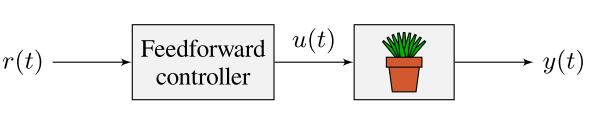
\includegraphics[width=0.7\textwidth]{Figure/开环控制系统.png}
	\caption{含前馈控制器的开环控制系统}
	\label{fig:open-loop}
\end{figure}

\begin{definition}[闭环系统]
	包含从对象输出反馈的信息的控制器称为\emph{闭环系统}或\emph{反馈控制器}。
\end{definition}

\begin{figure}[htbp]
	\centering
	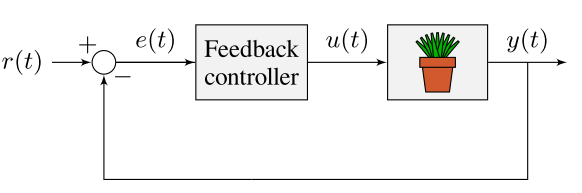
\includegraphics[width=0.7\textwidth]{Figure/闭环控制系统.png}
	\caption{闭环（反馈）控制系统}
	\label{fig:closed-loop}
\end{figure}

\begin{note}
	系统的输入和输出是从 \emph{plant} 的角度定义的。图中所示的负反馈控制器将基准与输出之间的差值，即误差变为 $0$。
\end{note}

\section{前馈}
反馈控制可以有效地用于基准跟踪（使系统的输出跟随期望的参考信号），但它是一种反应性措施；直到系统已经落后时，系统才会开始努力工作😭。

前馈控制器注入有关系统动态的信息或期望的运动。前馈控制器处理控制动作的一部分。前馈控制器注入有关系统动态或所需运动的信息。前馈处理我们已经知道必须应用的控制操作的一部分，以使系统跟踪引用，然后反馈补偿我们在运行时不知道或不能知道的系统行为。

有两种类型的前馈：
\begin{enumerate}
	\item 基于模型的前馈；
	\item 用于未建模动态的前馈。
\end{enumerate}
第一个是求解满足所需速度和加速度所需输入的系统的数学模型。

第二个直接补偿未建模的力或行为，因此反馈控制器没有必要进行操作。

这两种类型都可以使反馈控制器更简单。
